\section{BioMérieux Solution}

\begin{figure}[h]
    \centering
    
\includegraphics[scale=0.5]{img/bmx.png}
    \caption{Logo de bioMérieux}
\end{figure}

BioMérieux est une entreprise spécialisée dans le diagnostic in vitro et dans la microbiologie.
Cette entreprise concoit et fabrique des instruments permettant de diagnostiquer des maladies et de faire des analyses microbiologiques.
BioMérieux dispose d'un showroom permettant de montrer leur produits à leurs futurs clients.

\subsection{Situation initial}

Dans ce Showroom, un ensemble de dispositifs interactifs sont mis en place pour presenter les produits et l'entreprise.
Parmis ces équipements, on retrouve l'espace solution.
Cet espace présente un exemplaire physique des principales machines concus par BioMérieux.
Un projecteur permet alors d'afficher une image sur une vitre opacifiante.
L'image projetée est l'écran d'un Mac Mini disposé dans la salle technique du Showroom;
On utilise un lidar\footnote{Le lidar est un laser rotatif permettant, par balayage, de detecter la position d'un element dans l'espace.} pour reperer l'emplacement du doigt sur la vitre et ainsi controler l'ordinateur.

L'application présente avant ma mission etait développée en C++ avec OpenFrameworks\footnote{OpenFrameworks est un framework se basant sur de nombreuses librairies permettant la creation simplifiée d'applications graphiquement poussées. Il est très utilisé dans le domaine de la scenographie et du creative coding.}.
Cette application présente un arbre de composents graphiques chacun affichant un élément de l'interface.
Ce système, bien que fonctionnel, est assez peux flexible au regard des nouvelles fonctionnalités demandés par BioMérieux.

En effet, bioMérieux à recemment changé son logo et sa charte graphique pour un aspect plus épuré et flat-design\footnote{Le flat-design est un courant de design moderne qui possède une approche minimaliste de l'interface en se basant sur des aplats de couleurs unis et des effets d'ombres.}.
Pour reflèter ce changement dans leur showroom, l'entreprise a demandé un redesign de l'application.
De plus, pour pouvoir gèrer par eux même les produits presents dans l'application, bioMérieux a demandé la mise en place d'un backoffice qui permettra d'éditer le contenu de l'application sans faire appel à LTBL .

\begin{figure}[h]
    \centering
    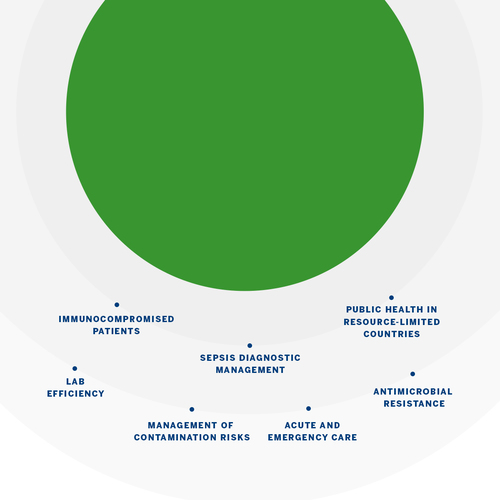
\includegraphics[scale=0.195]{img/resized-bmx-1-new.jpg}
    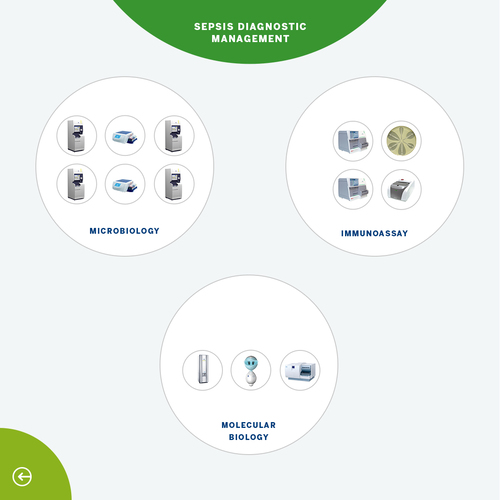
\includegraphics[scale=0.195]{img/resized-bmx-2-new.jpg}
    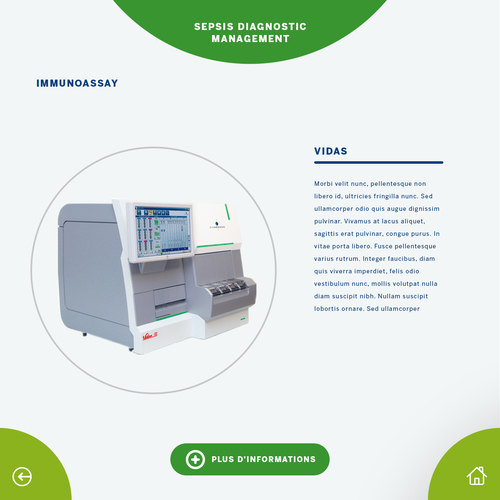
\includegraphics[scale=0.195]{img/resized-bmx-3-new.jpg}
    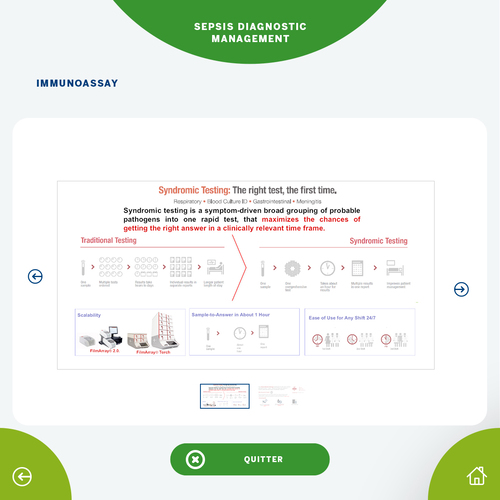
\includegraphics[scale=0.195]{img/resized-bmx-4-new.jpg}
    \caption{Design renouvelé de l'application Biomérieux}
\end{figure}

Enfin, dans une optique de recherche et développement d'une soltion universelle de backoffice chez LTBL il fallait aussi réfléchir à un système flexible de stockage de données.

Pour résumer, les fonctionnalités demandés sont :

\begin{itemize}
    \item La mise à jour de la charte graphique de bioMérieux
    \item La mise en place d'un backoffice pour gèrer les produits
    \item Faire en sorte que le backoffice puisse être réutilisé dans d'autres projets LTBL
\end{itemize}


\subsection{Conception de la solution}

Le code précédent étant totalement fait main, il est peu flexible et sensible aux bugs de développement.
De plus les données sont directement integrés dans le code et il serait chronophage et peu rentable de modifier cette application pour qu'elle d'adapte aux nouveaux besoins.
J'ai donc décide de reprendre l'application depuis le début et de choisir une solution technique qui me semble plus adaptée à une interface.

Pour ce projet, j'ai utilisé \emph{Electron} qui permet de créer des interfaces facilement à l'aide des technologies Web.
Je m'y penche plus en détails dans la partie suivante.

Pour le stockage des données, j'ai opté pour une base de données \emph{SQLite} permettant un stockage dans un fichier sans serveur superflu.
En effet, SQLite est une librairie C mettant à disposition un langage SQL et un stockage de données dans un fichier.
Cette technique est très intéressante dans notre cas, car les données ne seront qu'utilisées par l'application.
De plus, l'application ne nécessite pas de grandes performances et donc pas d'optimisation particulière que peuvent présenter les serveurs SGBDR\footnote{Système de Gestion de Bases de Données relationnelles} comme MariaDB ou PostgreSQL\@.

Enfin, pour gérer ces données j'utilise \emph{Sequelize}, un ORM JavaScript permettant de communiquer avec la base de données.
Cette librairie permet de représenter les données sous forme d'objets JavaScript pour éviter d'écrire les requêtes à la main et ainsi avoir une meilleure intégration des données dans l'environnement JavaScript.

\subsubsection{Electron}

Pour développer l'application j'ai décidé d'utiliser Electron.

\begin{figure}[h]
    \centering
    
\includegraphics[scale=0.2]{img/electron.png}
    \caption{Logo de Electron}
\end{figure}

Electron est un framework permttant de concevoir des application natives en utilisant les technologies web.
Electron embarque le moteur de rendu et le moteur Javascript de Chromium mais ajoute les fonctionalités de NodeJS permettant d'interagir avec le système hote.
Chromium est l'un des navigateurs les plus avencés dans l'integration des nouvelles normes et cela permet de profiter de nouvelles fonctionnalités très interessantes comme les Webcomponents et WebGL .
Enfin, on peut toujours accèder au système de fichiers de l'utilisateur et faire de la dépendances de modules NodeJS avec les fonctionnalités que propose Electron en plus des fonctionnalités de base que l'on retrouve sur un site web classique.

L'utilisation de ce framework est interessante dans le cas de cette application car elle permet de concevoir des interfaces simplement.
De plus, les langages web sont spécifiquement dédiés a la creation d'interfaces comme demandé.
Ainsi, on peut etimer que recoder l'application avec un nouveau design et le nouvelles fonctionnalités prendrais moins de temps que d'adapter l'ancienne application.

\subsection{WebComponents}

Le système de Webcomponents est un ensemble de nouvelles normes mises en place il y a peu de temps par le W3C et implémentés dans Chromium permettant de créer de nouveaux tags HTML avec des fonctionnalités spécifiques et isolés du reste de l'archithecture de la page.

Un Webcomponent est basé sur 4 normes :

\paragraph{Custom Elements} Une fonctionnalité permettant de créer un tag HTML personnalisé et reconnu par le navigateur comme faisant référence au code fournis.

\paragraph{HTML Template} Le tag \texttt{<template>} permet de créer un élément qui ne sera pas visible par l'utilisateur mais qui servira de squelette pour la creation de futurs éléments.
Dans les Webcomponents, on les utilisent pour créer le squelette de base de notre components.

\paragraph{Shadow DOM} Un concept permettant d'isoler une partie de l'arborescense d'une page Web.
Cela impliqe l'isolation du style et des éléments et cette technologie sert à créer le contenu caché de notre futur élément qui apparaitra comme une blackbox.

\paragraph{HTML Import} Permet d'importer un fichier HTML sans devoir inclure le HTML dans le document chargé au départ.
Cela permet notemment d'inclure tout le code HTML, CSS et JS d'un component dans un même fichier HTML.
Il suffira ensuite d'importer cet unique fichier HTML pour pouvoir utiliser le component.

\bigskip

Le développement en Webcomponent présente de nombreux avantages.
L'isolation du style CSS dans le Shadow DOM permet de ne pas provoquer de conflit CSS lors d'une séléction un peu trop générale sur le fichier de styles de base.
L'isolation du javascript permet de se concentrer uniquement sur le composant sans interferer avec le reste de l'application.
Enfin, l'approche unitaire des Webcomponents permet une réusablitié importante.

Mais l'approche par component pose aussi des difficultés.
En effet, il faut penser le composent en tant qu'élément générique.
Si on fait un composent trop spécifique ou dépendant de ses voisins, il sera difficile de réutiliser le composant dans un autre contexte de celui pour lequel il etait prévu au début.
Cela implique de réfléchir à la structure de l'application en amont et de changer la conception que l'on se fait d'une application.
Il ne faut plus penser l'application dans son ensemble mais comme une ensemble de blocs réutilisables ajoutés les uns aux autres.

Faire un bloc réutilisable passe par l'utilisation des attributs HTML comme vecteurs de transmission d'informations.
Mais aussi l'utilisation d'évennements Javascript comme vecteur de signal pour avertir les parents.

\bigskip

Dans ce projet, j'ai été amené à découvrir cette nouvelle norme du W3C par le biais des employés de l'entreprise qui utilisaient dàja cette technologie.
J'ai découvert les webcomponents et ai expériment avec ceux ci durant ce projet.
J'ai eu l'occasion, par le suite, d'affiner mes connaissances sur le sujet dans le cadre des 4 autres projets qui les utilisaient.

\subsection{Structure}

Pour cette structure, j'ai puisé dans mes connaissances acquises durant ma formation pour concevoir un système en 3 blocs.

\paragraph{Modèle} Le bloc de modèle définissant les données à stocker dans une base de données relationnelle standard.
Pour ce faire, j'utilise la librairie d'ORM \emph{Sequelize} ayant pour avantage d'être compatible avec la majeure partie des bases de données relationnelles actuelles.
Dans cet ORM, on doit définir un modèle, ce modèle sera utilisé pour créer les tables de la base de données.
Le modèle est donc défini dans un unique fichier \texttt{model.js} permettant de centraliser leurs déclarations.

\paragraph{Backoffice} Le back-office est un serveur web exécuté au sein de l'application Electron.
Ce serveur web se base sur le modèle pour créer les formulaires de saisie des données.
Le back-office ne présente aucun code spécifique au modèle de biomérieux, mais met en place une arborescence de formulaires générés en fonction du modèle défini par le développeur.
Cette technique permet de réutiliser ce back-office dans un tout autre contexte.
En effet, il suffit de changer le modèle pour que les formulaires de saisie changent dans le back-office.

\paragraph{Affichage client} L'affichage client représente tout ce qui va être affiché par l'application Electron sur le terminal.
Cet affichage est le seul qui sera vu par les visiteurs du showroom.
Dans l'architecture utilisée, c'est la seule partie spécifique.
Dans cette partie, on utilise les WebComponents pour concevoir l'application.

Parmi ces WebComponents, j'en ai créé des génériques permettant d'effectuer des tâches de base.
Ces WebComponents génériques sont donc :
\begin{itemize}
    \item \texttt{<data-element>} permettant de faire une requête dans la base de données s'actualisant à chaque changement
    \item \texttt{<page-router>} permettant d'afficher ou non une page en fonction de l'URL associée
    \item \texttt{<animation-block>} permettant d'animer des éléments de l'interface en utilisant les transitions CSS
\end{itemize}


\begin{figure}[h]
    \centering
    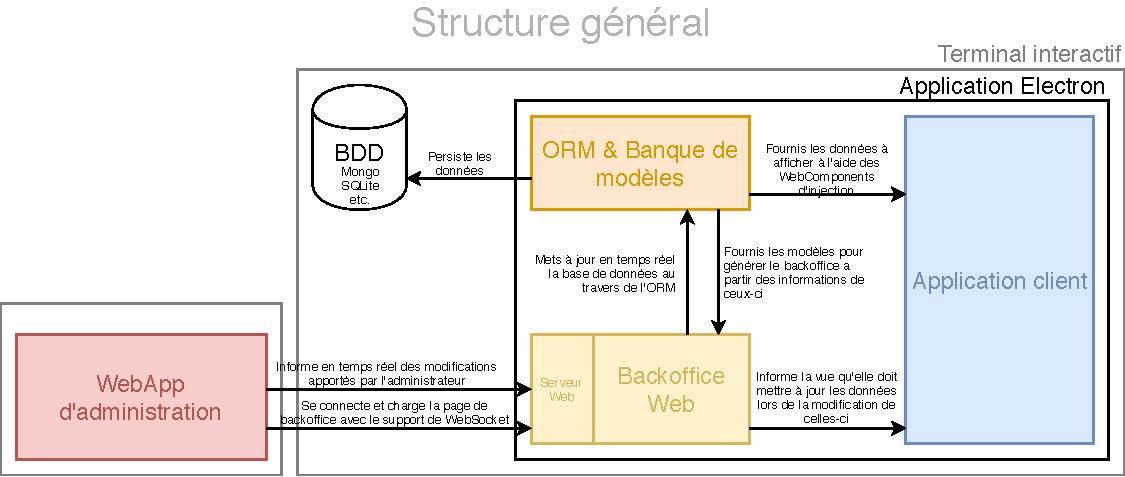
\includegraphics[scale=0.6]{img/Proposition-utopia.pdf}
    \caption{Structure générale de l'application Biomérieux}
\end{figure}